
We now consider the scenario where we have data from multiple patients and fit a population model.
Population models are a powerful tool to capture the heterogeneity between patients, while also recognizing similarities.
Building the right prior allows us to pool information between patients, the idea being that what we learn from one patient teaches us something -- though not everything -- about the other patients.
In practice, such models can frustrate inference algorithms and need to be implemented with care \cite[e.g.][]{Betancourt:2013}.
We start with an example where the interaction between the model and our MCMC sampler is well behaved.
In Part II of this tutorial, we will examine a more difficult case, for which we will leverage Stan's diagnostic capabilities in order to run reliable inference.

\subsection{Statistical model} \label{sec:twoCptPop_stat}

Let $\vartheta$ be the 2D array of body weight-normalized pharmacokinetic parameters for each patient,
with
\begin{equation*}
  \vartheta_j = (CL_{\mathrm{norm}, j}, Q_{\mathrm{norm}, j}, V_{\mathrm{cent}, \mathrm{norm},  j}, V_{\mathrm{peri}, \mathrm{norm}, j}, k_{a, j}),
\end{equation*} 
the parameters for the $j^\mathrm{th}$ patient.
We construct a population model by introducing random
variation to describe otherwise unexplained inter-individual
variability. In a Bayesian context this is sometimes referred to as a
prior distribution for the individual parameters.
\begin{eqnarray*}
  \log \vartheta_j \sim \mathrm{Normal} (\log \vartheta_\mathrm{pop}, \Omega),
\end{eqnarray*}
As before we work on the log scale to account for the fact the pharmacokinetic parameters are constrained to be positive.
$\vartheta_\mathrm{pop} = (CL_\mathrm{pop}, Q_\mathrm{pop}, V_\mathrm{cent, pop}, V_\mathrm{peri, pop}, k_\mathrm{a, pop})$ is the population mean and $\Omega$ the population covariance matrix.
Both $\vartheta_\mathrm{pop}$ and $\Omega$ are estimated.
% Prior information about the physiological parameters can now be encoded into priors on the population parameters, rather than on the individual parameters.
In this example, we start with the simple case where $\Omega$ is
diagonal.
For our example we will also use conventional allometric scaling to
adjust the clearance and volume parameters for body weight.
\begin{align*}
  CL_j &= CL_{\mathrm{norm}, j} \frac{\mathrm{weight}}{70}^{0.75} = \vartheta_{1j} \frac{\mathrm{weight}}{70}^{0.75} \\
  Q_j &= Q_{\mathrm{norm}, j} \frac{\mathrm{weight}}{70}^{0.75} = \vartheta_{2j} \frac{\mathrm{weight}}{70}^{0.75} \\
  V_{\mathrm{cent}, j} &= V_{\mathrm{cent}, \mathrm{norm},  j} \frac{\mathrm{weight}}{70} = \vartheta_{3j} \frac{\mathrm{weight}}{70}^{0.75} \\
  V_{\mathrm{peri}, j} &= V_{\mathrm{peri}, \mathrm{norm},  j} \frac{\mathrm{weight}}{70} = \vartheta_{4j} \frac{\mathrm{weight}}{70}^{0.75}
\end{align*}

The likelihood remains mostly unchanged, with the caveat that it must now be computed for each patient.
Putting this all together, we have the following model, as specified by the joint distribution,
\begin{eqnarray*}
  \vartheta_\mathrm{pop} & \sim & p(\vartheta_\mathrm{pop}), \hspace{1in} \text{(prior on pharmacokinetic parameters)} \\
  \Omega & \sim & p(\Omega), \hspace{1.2in} \text{(prior on population covariance)} \\
  \sigma & \sim & p(\sigma) \\
  \vartheta \mid \vartheta_\mathrm{pop}, \Omega  & \sim  & \mathrm{logNormal}(\vartheta_\mathrm{pop}, \Omega), \\
  \log y \mid c, \sigma & \sim & \mathrm{Normal}(\log c, \sigma).
\end{eqnarray*}

\subsection{Specifying the model in Stan}

We begin by adjusting our parameters block:
\begin{lstlisting}[style=stan, numbers=none]
parameters {
  // Population parameters
  real<lower = 0> CL_pop;
  real<lower = 0> Q_pop;
  real<lower = 0> VC_pop;
  real<lower = 0> VP_pop;
  real<lower = 0> ka_pop;

  // Inter-individual variability
  vector<lower = 0>[5] omega;
  real<lower = 0> theta[nSubjects, 5];

  // residual variability
  real<lower = 0> sigma;
}
\end{lstlisting}
%
The variable, $\vartheta_\mathrm{pop}$ is introduced in \texttt{transformed parameters},
mostly for convenience purposes:
\begin{lstlisting}[style=stan, numbers=none]
vector<lower = 0>[nTheta]  
  theta_pop = to_vector({CL_pop, Q_pop, VC_pop, VP_pop, 
                         ka_pop});
\end{lstlisting}
%
The model block reflects our statistical formulation:
\begin{lstlisting}[style=stan, numbers=none] 
model {
  // prior on population parameters
  CL_pop ~ lognormal(log(10), 0.25); 
  Q_pop ~ lognormal(log(15), 0.5);
  VC_pop ~ lognormal(log(35), 0.25);
  VP_pop ~ lognormal(log(105), 0.5);
  ka_pop ~ lognormal(log(2.5), 1);
  omega ~ lognormal(0.25, 0.1);
  
  sigma ~ normal(0, 1);

  // interindividual variability
  for (j in 1:nSubjects)
    theta[j, ] ~ lognormal(log(theta_pop), omega);

  // likelihood
  cObs ~ lognormal(log(concentrationObs), sigma);
}
\end{lstlisting}
%

In the \texttt{transformed parameters} lock we also declare and
calculate the individual parameters given $\vartheta_j$ and any
relevant covariates---body weight in this case.
\begin{lstlisting}[style=stan, numbers=none] 
  // Individual parameters
  vector<lower = 0>[nSubjects] CL = to_vector(theta[, 1]) .* exp(0.75 * log(weight / 70 ));
  vector<lower = 0>[nSubjects] Q = to_vector(theta[, 2]) .* exp(0.75 * log(weight / 70 ));
  vector<lower = 0>[nSubjects] VC = to_vector(theta[, 3]) .* (weight / 70);
  vector<lower = 0>[nSubjects] VP = to_vector(theta[, 4]) .* (weight / 70);
  vector<lower = 0>[nSubjects] ka = to_vector(theta[, 5]);
\end{lstlisting}

It remains to compute \texttt{concentrationObs}.
There are several ways to do this and, depending on the computational resources available, we may either compute the concentration for each patients sequentially or in parallel.
For now, we do the simpler sequential approach.
In the upcoming Part II of this tutorial, we examine how Torsten offers easy-to-use parallelization  for population models.

Sequentially computing the concentration is a simple matter of bookkeeping.
In \texttt{transformed parameters} we loop through the patients using a \texttt{for} loop.
The code is identical to what we used in Section~\ref{sec:twocpt_transformed_parameters},
with the caveat that the arguments to \texttt{pmx\_solve\_twocpt} are now indexed to indicate for which patient we compute the drug mass.
For example, assuming the time schedule is ordered by patient, the event times corresponding to the $j^\mathrm{th}$ patient are given by
\begin{lstlisting}[style=stan, numbers=none]
time[start[j]:end[j]]
\end{lstlisting}
%
where \texttt{start[j]} and \texttt{end[j]} contain the indices of the first and last event for the $j^\mathrm{th}$ patient, and the syntax for indexing is as in R.
The full \texttt{for} loop is then
%
\begin{lstlisting}[style=stan, numbers=none]
for (j in 1:nSubjects) {
  mass[, start[j]:end[j]] = pmx_solve_twocpt(time[start[j]:end[j]],
                                             amt[start[j]:end[j]],
                                             rate[start[j]:end[j]],
                                             ii[start[j]:end[j]],
                                             evid[start[j]:end[j]],
                                             cmt[start[j]:end[j]],
                                             addl[start[j]:end[j]],
                                             ss[start[j]:end[j]],
                                             {CL[j], Q[j], VC[j], VP[j], ka[j]});

  concentration[start[j]:end[j]] = 
                    mass[2, start[j]:end[j]] / VC[j];
}
\end{lstlisting}

Once we have written our Stan model, we can apply the same methods for inference and diagnostics as we did in the previous section.

\subsection{Posterior predictive checks}

We follow the exact same procedure as in Section~\ref{sec:twoCpt_ppc} -- using even the same line of code -- to create new observations for our patients.
Figure~\ref{fig:twoCptPop_ppc} plots the results across patients.
In addition, we simulate data for new patients by: (i) drawing pharmacokinetic parameters from our population distribution, (ii) solving the ODEs with these simulated parameters and (iii) using our measurement model to simulate new observations.
The generated quantities block then looks as follows:
%
\begin{lstlisting}[style=stan, numbers=none]
generated quantities {
  real concentrationObsPred[nObs] 
    = exp(normal_rng(log(concentration[iObs]), sigma));

  real cObsNewPred[nObs];
  matrix<lower = 0>[nCmt, nEvent] massNew;
  real thetaNew[nSubjects, nTheta];
  row_vector<lower = 0>[nEvent] concentrationNew;
  vector<lower = 0>[nSubjects] CLNew;
  vector<lower = 0>[nSubjects] QNew;
  vector<lower = 0>[nSubjects] VCNew;
  vector<lower = 0>[nSubjects] VPNew;
  vector<lower = 0>[nSubjects] kaNew;

  for (j in 1:nSubjects) {
    thetaNew[j, ] = lognormal_rng(log(theta_pop), omega);

  CLNew = to_vector(thetaNew[, 1]) .* exp(0.75 * log(weight / 70 ));
  QNew = to_vector(thetaNew[, 2]) .* exp(0.75 * log(weight / 70 ));
  VCNew = to_vector(thetaNew[, 3]) .* (weight / 70);
  VPNew = to_vector(thetaNew[, 4]) .* (weight / 70);
  kaNew = to_vector(thetaNew[, 5]);

  massNew[, start[j]:end[j]]
      = pmx_solve_twocpt(time[start[j]:end[j]],
                      amt[start[j]:end[j]],
                      rate[start[j]:end[j]],
                      ii[start[j]:end[j]],
                      evid[start[j]:end[j]],
                      cmt[start[j]:end[j]],
                      addl[start[j]:end[j]],
                      ss[start[j]:end[j]],
                      {CLNew[j], QNew[j], VCNew[j], VPNew[j], kaNew[j]});

      concentrationNew[start[j]:end[j]]
        = massNew[2, start[j]:end[j]] / VCNew[j];
  }

  cObsNewPred = lognormal_rng(log(concentrationNew[iObs]), sigma);
}
\end{lstlisting}

\begin{figure}
  \begin{center}
  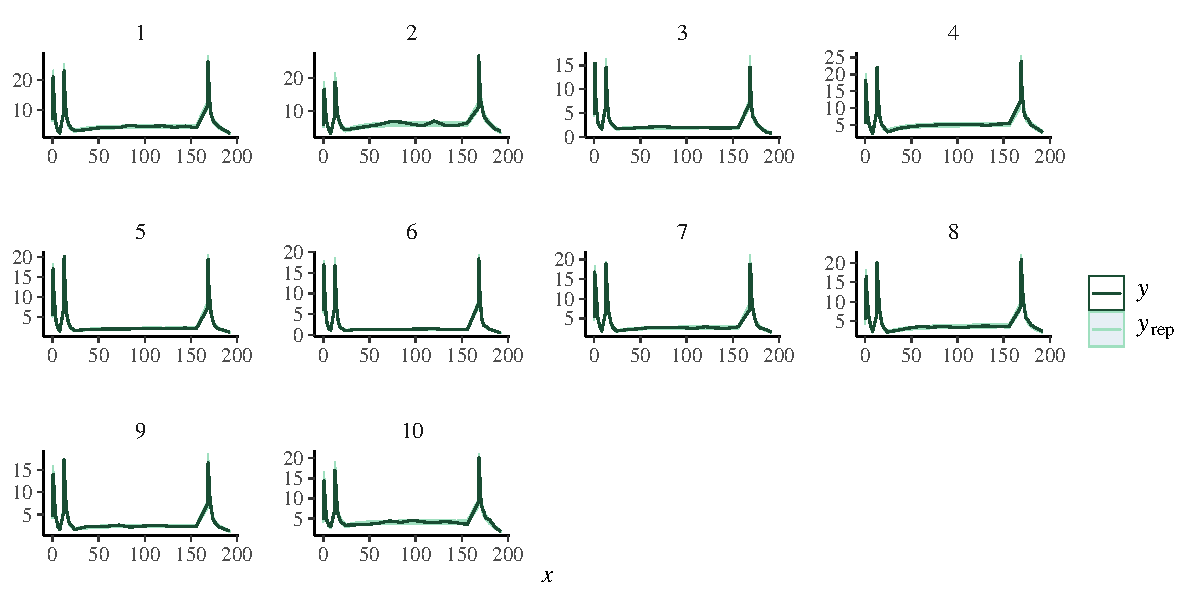
\includegraphics[width=6in]{../figures/twocpt_pop_ppc_4x8.pdf}
  \end{center}
  \caption{Posterior predictive checks for population two compartment model.}
  \label{fig:twoCptPop_ppc}
\end{figure}

It is worth noting that the computational cost of running operations in the \texttt{generated quantities} is relatively small.
While these operations are executed once per iteration, in order to generate posterior samples of the generated quantities, operations in the \texttt{transformed parameters} and \texttt{model} blocks are run and differentiate multiple times per iterations, meaning they amply dominate the computation.
Hence the cost of doing posterior predictive checks, even when it involves solving ODEs, is marginal.
The computational scaling of Stan, notably for ODE-based models, is discussed in the article by \citet{Grinsztajn:2021}.
